%besoin en entrée à méthode « agile » - \\
%description de la méthode – \\
%application et différence par rapport // DTI +\\
%enrichir le produit si cela marche\\
%Avantage/inconvénient Extreme programming :\\
%Revue logicielle (validations qui permettront de faire évoluer le produit)
\section{Gestion de projet}
    \subsection{Choix de la méthode de gestion de projet}
Comme nous l'avons vu précédemment, les besoins ne sont pas clairement définis dès le début. Il était donc difficile de pouvoir établir des spécifications explicites dans le but de mettre en place un cycle en V \nref{cyclev}. Nous avons donc choisis une méthodologie de gestion de projet différente de celle appliquée en temps normal à la \textsc{Dti}.

Cette méthodologie devait nous permettre de débuter un projet sans en connaître réellement l'aboutissement final tout en gardant de la rigueur et de l'organisation. Nous avons donc décidé d'utiliser une méthode agile\footnote{Les méthodes Agiles sont des groupes de pratiques pouvant s'appliquer à divers types de projets, mais se limitant plutôt actuellement aux projets de développement en informatique (conception de logiciel). Les méthodes Agiles se veulent plus pragmatiques que les méthodes traditionnelles. Elles impliquent au maximum le demandeur (client) et permettent une grande réactivité à ses demandes. Elles visent la satisfaction réelle du besoin du client et non les termes d'un contrat de développement. }. Après quelques recherches et comparaisons nous nous sommes orientés sur l'extreme programming \nref{extreme}. Nous allons donc vous décrire cette méthodologie et la comparer avec le système utilisé habituellement.

    \subsection{L' Extreme Programming\label{extreme}}

\begin{figure}[!h]
\center
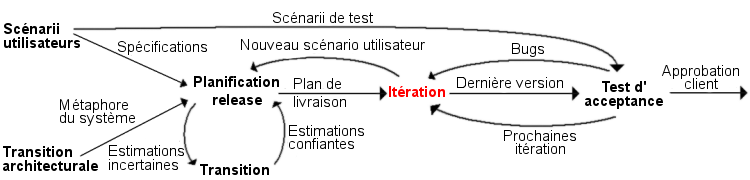
\includegraphics[width=15cm]{images/xp.png}
\caption{Cycle de l'Exreme Programing.}
\label{XP}
\end{figure}

L'Extreme Programming a été inventée par Kent Beck, Ward Cunningham et Ron Jeffries pendant leur travail sur un projet « C3 » de calcul des rémunérations chez Chrysler. Kent Beck, chef de projet en mars 1996 commença à affiner la méthodologie de développement utilisée sur le projet. La méthode est née officiellement en octobre 1999 avec le livre Extreme Programming Explained de Kent Beck. "Wikipedia".

Dans les méthodes traditionnelles, les besoins sont définis et souvent fixés au départ du projet, ce qui accroît les coûts ultérieurs de modifications. Extreme programming s'attache à rendre le projet plus flexible et ouvert au changement en introduisant des valeurs de base, des principes et des pratiques.

L'Extreme Programming repose sur des cycles rapides de développement (des itérations de quelques semaines voir dans notre cas quelques jours seulement) dont les étapes sont les suivantes:
\begin{itemize}
\item une phase d'exploration détermine les scénarios clients qui seront fournis pendant cette itération,
\item la transformation des scénarios en tâches à réaliser et en tests fonctionnels,
\item lorsque tous les tests fonctionnels passent, le produit est livré.
\end{itemize}\medskip

Lorsqu'une tâche est terminée, les modifications sont immédiatement intégrées dans le produit complet. On évite ainsi la surcharge de travail liée à l'intégration de tous les éléments avant la livraison. Les tests facilitent grandement cette intégration: quand tous les tests passent, l'intégration est terminée.

Le cycle se répète tant que le client peut fournir des scénarios à livrer (cf. Fig. \vref{XP}). Généralement le cycle de la première livraison se caractérise par sa durée et le volume important de fonctionnalités embarquées. Après la première mise en production, les itérations peuvent devenir plus courtes (par exemple la séparation des plans de vol en catégories tel que: transit, interne ...)

Pour résumer, cette méthode nous amène à réaliser la boucle suivante:
\begin{itemize}
\item Analyse du besoin
\item Expression des spécifications
\item Réalisation technique
\item Test de la réalisation
\item Revue logicielle (validations qui permettront de faire évoluer le produit)
\end{itemize}\medskip

    \subsection{Le cycle en V}

\begin{figure}[!h]
\center
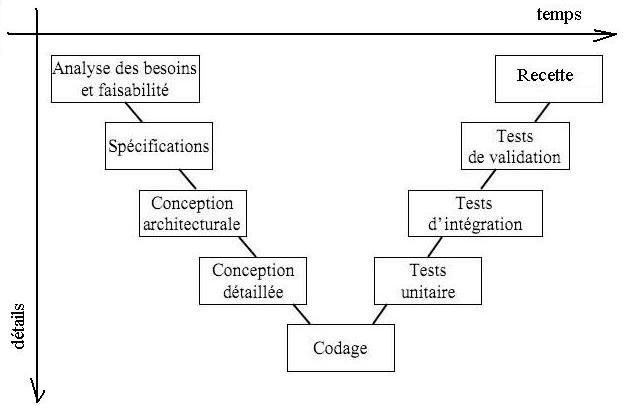
\includegraphics[width=12cm]{images/cyclev.png}
\caption{Les phases à travers le temps et le niveau de détails.}
\label{cyclev}
\end{figure}

Le modèle du cycle en V est un modèle conceptuel de gestion de projet étudié pour résoudre le problème de réactivité du modèle en cascade. Il permet, en cas d'anomalie, de limiter un retour aux étapes précédentes. Les phases \figref{cyclev} de la partie montante doivent renvoyer de l'information sur les phases en vis-à-vis lorsque des défauts sont détectés, afin d'améliorer le logiciel.

Le cycle en V est devenu un standard de l'Industrie logicielle depuis les années 1980 et depuis l'apparition de l'Ingénierie des Systèmes est devenu un standard conceptuel dans tous les domaines de l'Industrie. Le monde du logiciel ayant de fait pris un peu d'avance en termes de maturité, on trouvera dans la bibliographie courante souvent des références au monde du logiciel qui pourront s'appliquer au système.

Les étapes qui constituent cette méthode sont les suivantes :
\begin{itemize}
    \item Analyse des besoins et faisabilité
    \item Spécification logicielle
    \item Conception architecturale
    \item Conception détaillée
    \item Codage
    \item Test unitaire
    \item Test d'intégration
    \item Test de validation (Recette Usine, Validation Usine - VAU)
    \item Recette (Vérification d'Aptitude au Bon Fonctionnement - VABF)
\end{itemize}\medskip
 
Dans notre cas, avec ces besoins indéfinis, cette méthodologie engendrerait un risque. Ce risque serait que le logiciel final ne fonctionne pas ou ne reponde pas aux attentes du client.

\subsection{Les avantages et inconvénients}
Pour notre cas, les avantages de cette méthode sont les suivants:
\begin{itemize}
    \item Enrichir le produit à chaque itération du cycle. Ci le logiciel est fonctionel, le client peut visualiser immédiatement les besoins qui étaient superficiels (dont il n'avait pas réellement besoin) et au contraire découvrir de nouveaux besoins.
    \item Rediriger rapidement la conduite du projet. Si le client souhaite rediriger son projet, ceci peut être fait dans les meilleurs délais (changement d'objectifs ou de priorités)
%    \item ... a completer.
\end{itemize}\medskip
 
Cette méthode implique tout de même un certain nombre d'inconvénients tels que:
\begin{itemize}
    \item Le client doit être disponible afin de faire avancer le projet. Chaque validation est vue avec le client et c'est celui-ci qui donne les nouveaux besoins. Ce qui implique que ci celui-ci n'est pas disponible, le projet peut vite être bloqué. 
    \item Le projet peut vite dériver. Ce type de méthode requiert des personnes compétentes, aussi bien au niveau Maitre d'ouvrage, qu'au niveau maitre d'œuvre. Il est facile de s'égarer c'est pourquoi une organisation et une rigueur doivent être entretenues tout au long du projet.
    \item Lors du début du projet, on manque cruellement de spécifications. On se lance alors dans le développement sans analyse complète.    
%    \item ... a completer.
\end{itemize}\medskip







    
